% !TEX root = EUDAQUserManual.tex
\section{Run an Example Setup}
This section will describe running the DAQ system, mainly from the point of view of running an example setup as a demonstration without dedicated hardware.
However, this description can be applied to a detector DAQ system in general.

\subsection{Target Setup}
In this example, a user hardware device is simulated and implemented as an example Producer which can be configured to generate fake data. This works similarly to a real Producer, but does not talk to any real hardware. An example DataCollector is also implemented. \\
The runtime setup consists of the following EUDAQ processes.
\begin{description}
\ttitem{RunControl}
Standard RunControl GUI.
\ttitem{LogCollector}
Standard LogCollector GUI.
\ttitem{Producer}
Two Producers instanced by the CLI command. One of them produces events at a rate of 1\,Hz, the other produces events at a rate of 2\,Hz.
\ttitem{DataCollector}
Two DataCollectors instanced by the CLI command. One of them receives events only from the Producer at a 1\,Hz rate, the other receives events from both Producers, and synchronises the two streams by a timestamp.
\ttitem{Monitor}
No monitor exists. (TODO: producer generate hit data)
\end{description}

\subsection{Preparation}
Some preparation is needed to make sure the environment is set up correctly and
the necessary TCP ports are not blocked before the DAQ can run properly.

\subsubsection{Directories}
If no specified path is passed to EUDAQ (by configuration file or command line parameter), EUDAQ will assume the working folder where executable is started up  is writable. Data and log files will be stored in the working folder.

\subsubsection{Init/Config-Files}\label{sec:ConfigFiles}
\texttt{$\ast$.ini}-files for initialization and \texttt{$\ast$.conf}-files for configuration
are text files in a specific format, containing name-value pairs separated into different sections.\footnote{\url{https://en.wikipedia.org/wiki/INI\_file}}
Any text from a \texttt{\#} character until the end of the line is treated as a comment, and
ignored.  
Each section in the config file is delimited by a name in square brackets
(e.g. \verb@[RunControl]@).  
The name represents the type of process to which it applies; if there
are several such processes, then they can be differentiated by including the name after a period
(e.g. \verb@[Producer.Example]@).  
Within each section, any number of parameters may be specified,
in the form \mbox{\texttt{Name = Value}}.  
It is then up to the individual processes how these parameters are interpreted.

During the initialization and configuration, each process gets its section and does not know about the other parts of the ini/conf files.
\myinputlisting[conf]{-30}{user/example/misc/Ex0.ini}

\myinputlisting[conf]{-30}{user/example/misc/Ex0.conf}

\subsubsection{Ports and Firewall}
The different processes communicate between themselves using TCP/IP sockets. The ports can be configured when calling the the processors on the command line (see below). By default, TCP port 44000 is listened to by the RunControl, and TCP port 44002 is listened to by the LogCollector to get connections from clients. The DataCollector will pick a random TCP port to listen to and get incoming data from its connected Producers if there is no specific port assigned explicitly by user.

When all EUDAQ processes run on the same computer, common firewalls will not affect the TCP connections among them. However, running EUDAQ distributively on several computers may have issue from firewall blocking. You will have to open up those TCP ports for incoming connections or temporally shut down the firewall. Shutting down the firewall is operating-system dependent.\\

In this example, all processes will run on the same Linux computer, so we can skip the setup of TCP port.

%%%%%%%%%%%%%%%%%%%%%%%%%%%%%%%%%%%%%%%%%%%%%%%%%%%%%%%%%%%%%%%55
\subsection{Startup}
To start EUDAQ, all of the necessary processes have to be started in the correct order.
The first process must be the Run Control (euRun),
since all other processes will attempt to connect to it when they start up.
Then it is recommended to start the Log Collector,
since any log messages it receives may be useful
to help with debugging in case everything does not start as expected.
Finally, the Data Collector, Producers and Monitor can be started.

\subsubsection{RunControl}
\label{sec:runcontrol}
There are two versions of the RunControl -- a text-based version \texttt{euCliRun} and a graphical version \texttt{euRun} (see \autoref{fig:RunControl}).

The command line pattern to start up a Log Collector is:
\begin{listing}[mybash]
$[euRun]$ -a tcp://{listening_port}
\end{listing}

\begin{description}
\ttitem{-a \param{listening\_addr}}
optional, \texttt{listening\_port} default value is 44000.
\end{description}

For this example setup, we will startup the GUI version of Run Control and make it serve at TCP port 44000:\\
\begin{listing}[mybash]
$[euRun]$ -a tcp://44000
\end{listing}

After executing the above command, a new GUI windows is shown in \autoref{fig:RunControl}.
\begin{figure}[htb]
  \begin{center}
    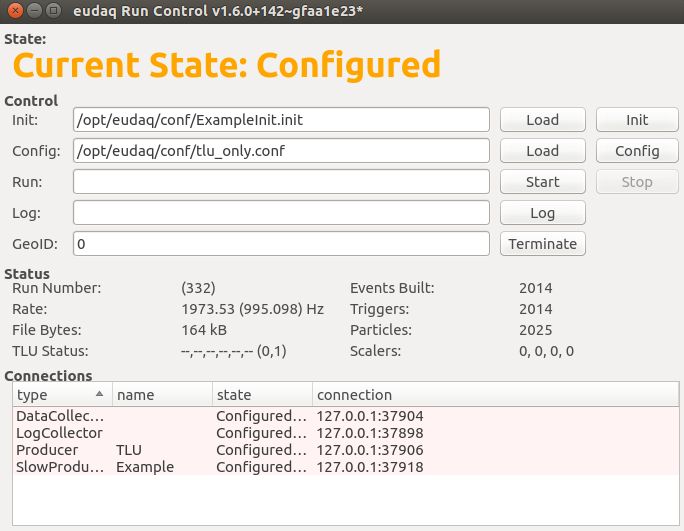
\includegraphics[width=0.8\textwidth]{src/images/RunControl}
    \caption{The Run Control graphical user interface.}
    \label{fig:RunControl}
  \end{center}
\end{figure}

\paragraph{Initialization Section}
none

\paragraph{Configuration Section}
\begin{listing}[conf]
[RunControl]
EventSizeLimit=10000
\end{listing}

\subsubsection{LogCollector}
\label{sec:logcollector}
It is recommended to start the Log Collector directly after having started the Run Control and before starting other processors in order to collect all log messages generated by all other processes.

There are also two versions of the Log Collector.
The graphical version is called \texttt{euLog},
and the text-based version is called \texttt{euCliLog}.

The command line pattern to startup a Log Collector is:
\begin{listing}[mybash]
$[euLog]$ -r tcp://{run_contorl_hostname}:{run_contorl_port} -a tcp://{listening_port}
\end{listing}

\begin{description}
\ttitem{-r \param{runcontrol\_addr}}
optional, \texttt{run\_control\_hostname} default value: localhost;  \texttt{run\_contorl\_port}  default value: 44000.
\ttitem{-a \param{listening\_addr}}
optional, \texttt{listening\_port} default value is 44002.
\end{description}

For this example setup, we will startup the GUI version of Log Collector, connect it to the Run Contorl at local port 44000 and make it serve at TCP port 44002:\\
\begin{listing}[mybash]
$[euLog]$ -r tcp://localhost:44000 -a tcp://44002
\end{listing}

After executing the above command, a new GUI window, as shown in \autoref{fig:LogCollector}, is opened and the RunControl displays a new connection, as seen in \autoref{fig:RunControl_con_log}.
\begin{figure}[htb]
  \begin{center}
    \includegraphics[width=\textwidth]{src/images/LogCollector}
    \caption{The Log Collector graphical user interface.}
    \label{fig:LogCollector}
  \end{center}
\end{figure}


\begin{figure}[htb]
  \begin{center}
    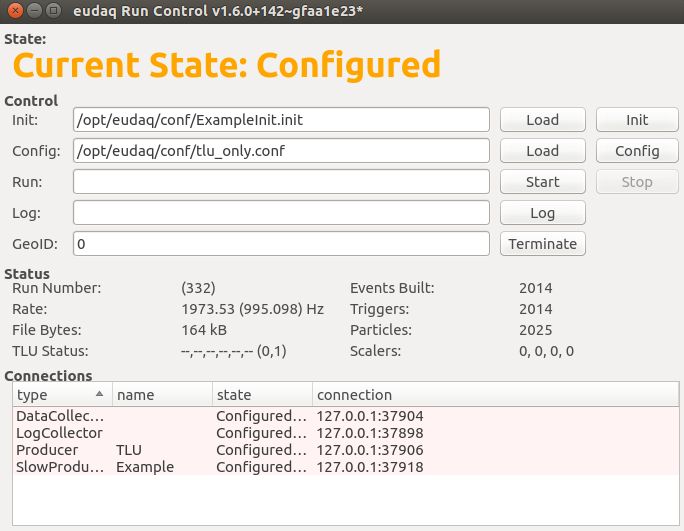
\includegraphics[width=0.8\textwidth]{src/images/RunControl}
    \caption{The Run Control with connection from Log Collector.}
    \label{fig:RunControl_con_log}
  \end{center}
\end{figure}


\subsubsection{DataCollector}
\label{sec:datacollector}
There is only a text-based version called \texttt{euCliDataCollector}.
The command line pattern to startup a DataCollector is:
\begin{listing}[mybash]
$[euCliDataCollector]$ -n {code_name} -t {runtime_name} -r tcp://{run_control_hostname}:{run_contorl_port} -a tcp://{listening_port}
\end{listing}

\begin{description}
\ttitem{-n \param{code\_name}}
required.
\ttitem{-t \param{runtime\_name}}
required.
\ttitem{-r \param{runcontrol\_addr}}
optional, \texttt{run\_control\_hostname} default value: localhost;  \texttt{run\_contorl\_port}  default value: 44000.
\ttitem{-a \param{listening\_addr}}
optional, \texttt{listening\_port} default value is random.
\end{description}

By default, an example DataCollector \texttt{Ex0TgDataCollector} is available with the standard installation of EUDAQ.
For this example setup, we will startup two instances of \texttt{Ex0TsDataCollector} with runtime names \texttt{my\_dc} and \texttt{another\_dc}\\
\begin{listing}[mybash]
$[euCliCollector]$ -n Ex0DataCollector -t my_dc -r tcp://localhost:44000 -a tcp://45001
$[euCliCollector]$ -n Ex0DataCollector -t another_dc -r tcp://localhost:44000 -a tcp://45002
\end{listing}

\paragraph{Initialization Section}
\begin{listing}[conf]
[DataCollector.my_dc]
KEY1=a

[DataCollector.another_dc]
KEY1=b
\end{listing}

\paragraph{Configuration Section}
Each Data Collector has to write to a different file by including the
\texttt{FilePattern} option in the corresponding section of your
configuration file (also see section \ref{sec:ConfigFiles}):

\begin{listing}[conf]
[DataCollector.my_dc]
FilePattern=run$6R$X

[DataCollector.another_dc]
FilePattern=dc2_run$6R$X
\end{listing}


\subsubsection{Producer}
\label{sec:testproducer}
There is only a text-based version called \texttt{euCliProducer}.
The command line pattern to startup a Producer is:
\begin{listing}[mybash]
$[euCliProducer]$ -n {code_name} -t {runtime_name} -r tcp://{run_control_hostname}:{run_contorl_port}
\end{listing}

\begin{description}
\ttitem{-n \param{code\_name}}
required.
\ttitem{-t \param{runtime\_name}}
required.
\ttitem{-r \param{runcontrol\_addr}}
optional, \texttt{run\_control\_hostname} default value: localhost;  \texttt{run\_contorl\_port}  default value: 44000.
\end{description}

By default, an example Producer \texttt{Ex0Producer} is available with the standard installation of EUDAQ.
For this example setup, we will startup two instances of \texttt{Ex0Producer} with runtime names \texttt{prd1hz} and \texttt{prd2hz}\\
\begin{listing}[mybash]
$[euCliProducer]$ -n Ex0Producer -t prd1hz -r tcp://localhost:44000
$[euCliProducer]$ -n Ex0Producer -t prd2hz -r tcp://localhost:44000
\end{listing}


After executing all of the above commands, the RunControl GUI window will be as in \autoref{fig:RunControl_1l2d2p}.

\begin{figure}[htb]
  \begin{center}
    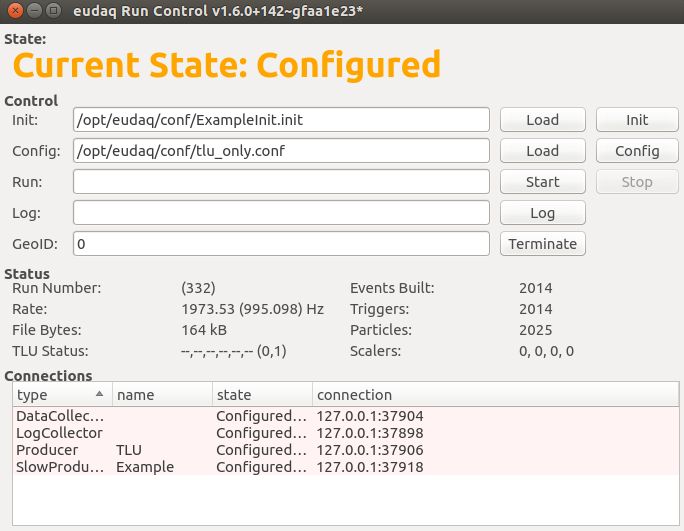
\includegraphics[width=0.8\textwidth]{src/images/RunControl}
    \caption{The RunControl with connections of two Producers.}
    \label{fig:RunControl_1l2d2p}
  \end{center}
\end{figure}

\paragraph{Initialization Section}
\begin{listing}[conf]
[Producer.prd1hz]
EUDAQ_DC=my_dc

[Producer.prd2hz]
EUDAQ_DC=my_dc,another_dc
\end{listing}

\paragraph{Configuration Section}
\begin{listing}[conf]
[Producer.prd1hz]
Rate=1
Random=true

[Producer.prd2hz]
Rate=2
Random=false
\end{listing}


\subsubsection{Monitor}
\label{sec:onlinemonitor}
There is a RootMonitor which can run in both online and offline modes.
To run it in online mode, the command line pattern is:
\begin{listing}[mybash]
$[OnlineMon]$ -r tcp://{run_control_hostname}:{run_contorl_port} -a tcp://{listenning_port}
\end{listing}

\begin{description}
\ttitem{-r \param{runcontrol\_addr}}
optional, \texttt{run\_control\_hostname} default value: localhost;  \texttt{run\_contorl\_port}  default value: 44000.
\ttitem{-a \param{listening\_addr}}
optional, \texttt{listening\_port} default value is random.
\end{description}

In offline mode, there is no Run Control, To run it in online mode, the command line pattern is:
\begin{listing}[mybash]
$[OnlineMon]$ -f {path_to_data_file}
\end{listing}

\begin{description}
\ttitem{-f \param{path\_to\_data\_file}}
required
\end{description}

%%\begin{figure}[htb]
%%  \begin{center}
%%    \includegraphics[width=0.8\textwidth]{src/images/OnlineMonCorrelations}
%%    \caption{The OnlineMon showing correlation plots between different
%%      Mimosa26 planes of the EUDET telescope.}
%%    \label{fig:OnlineMonPlots}
%%  \end{center}
%%\end{figure}

\subsection{Operating}
Once all the processes have been started, they report their status to the RunControl (see \autoref{fig:RunControl}).
Depending on their status, EUDAQ and all processes can be initialized, configured or re-configured, data taking (runs) can be started and stopped, and the software can be terminated.

\begin{itemize}
\item First, the appropriate initialization file should be selected (see \autoref{sec:ConfigFiles} for creating and editing init-files). Then the \texttt{Init} button can be pressed,
which will send an initialization command to all connected processes.

\item Second, the appropriate configuration should be selected 
  (see \autoref{sec:ConfigFiles} for creating and editing configurations).
%%%  ,
%%%and the \texttt{GeoID} should be verified, before continuing.
Then the \texttt{Config} button can be pressed,
which will send a configuration command
(with the contents of the selected configuration file) to all connected processes.
The full contents of the configuration file will also be stored
in the \gls{BORE} of the data file,
so that this information is always available along with the data.
\item Once all connected processes are fully configured, a run may be started, by pressing the \texttt{Start} button.
Whatever text is in the corresponding text box (``\texttt{Run:}'') when the button is pressed
will be stored as a comment in the data file.
This can be used to help identify the different runs later.
\item Once a run is completed, it may be stopped by pressing the \texttt{Stop} button.
Runs will also stop and restart automatically when the data file reaches a threshold in size (by default this is 1~GB).%
\footnote{This is because there is a file size limit of 2~GB for storage on the GRID,
and the processed files can be bigger than the original native files.}
The threshold size for restarting a run may be configured in the config file (see \autoref{sec:ConfigFiles}).
\item At any time, a message may be sent to the log file by filling in the (``\texttt{Log:}'') text box and pressing the corresponding button.
The text should appear in the LogCollector window, and will be stored in the log file for later access.
\item Once the run is stopped, the system may be reconfigured with a different configuration, or another run may be started; or EUDAQ can be terminated.
  
\end{itemize}
